\documentclass[border=10pt]{standalone}
\usepackage[svgnames]{xcolor}
\usepackage{amsmath}
\usepackage{pgfplots}
\pgfplotsset{compat=newest}
\usepackage[sfdefault]{FiraSans}
\usepackage{FiraMono}
\renewcommand*\familydefault{\sfdefault}
\begin{document}
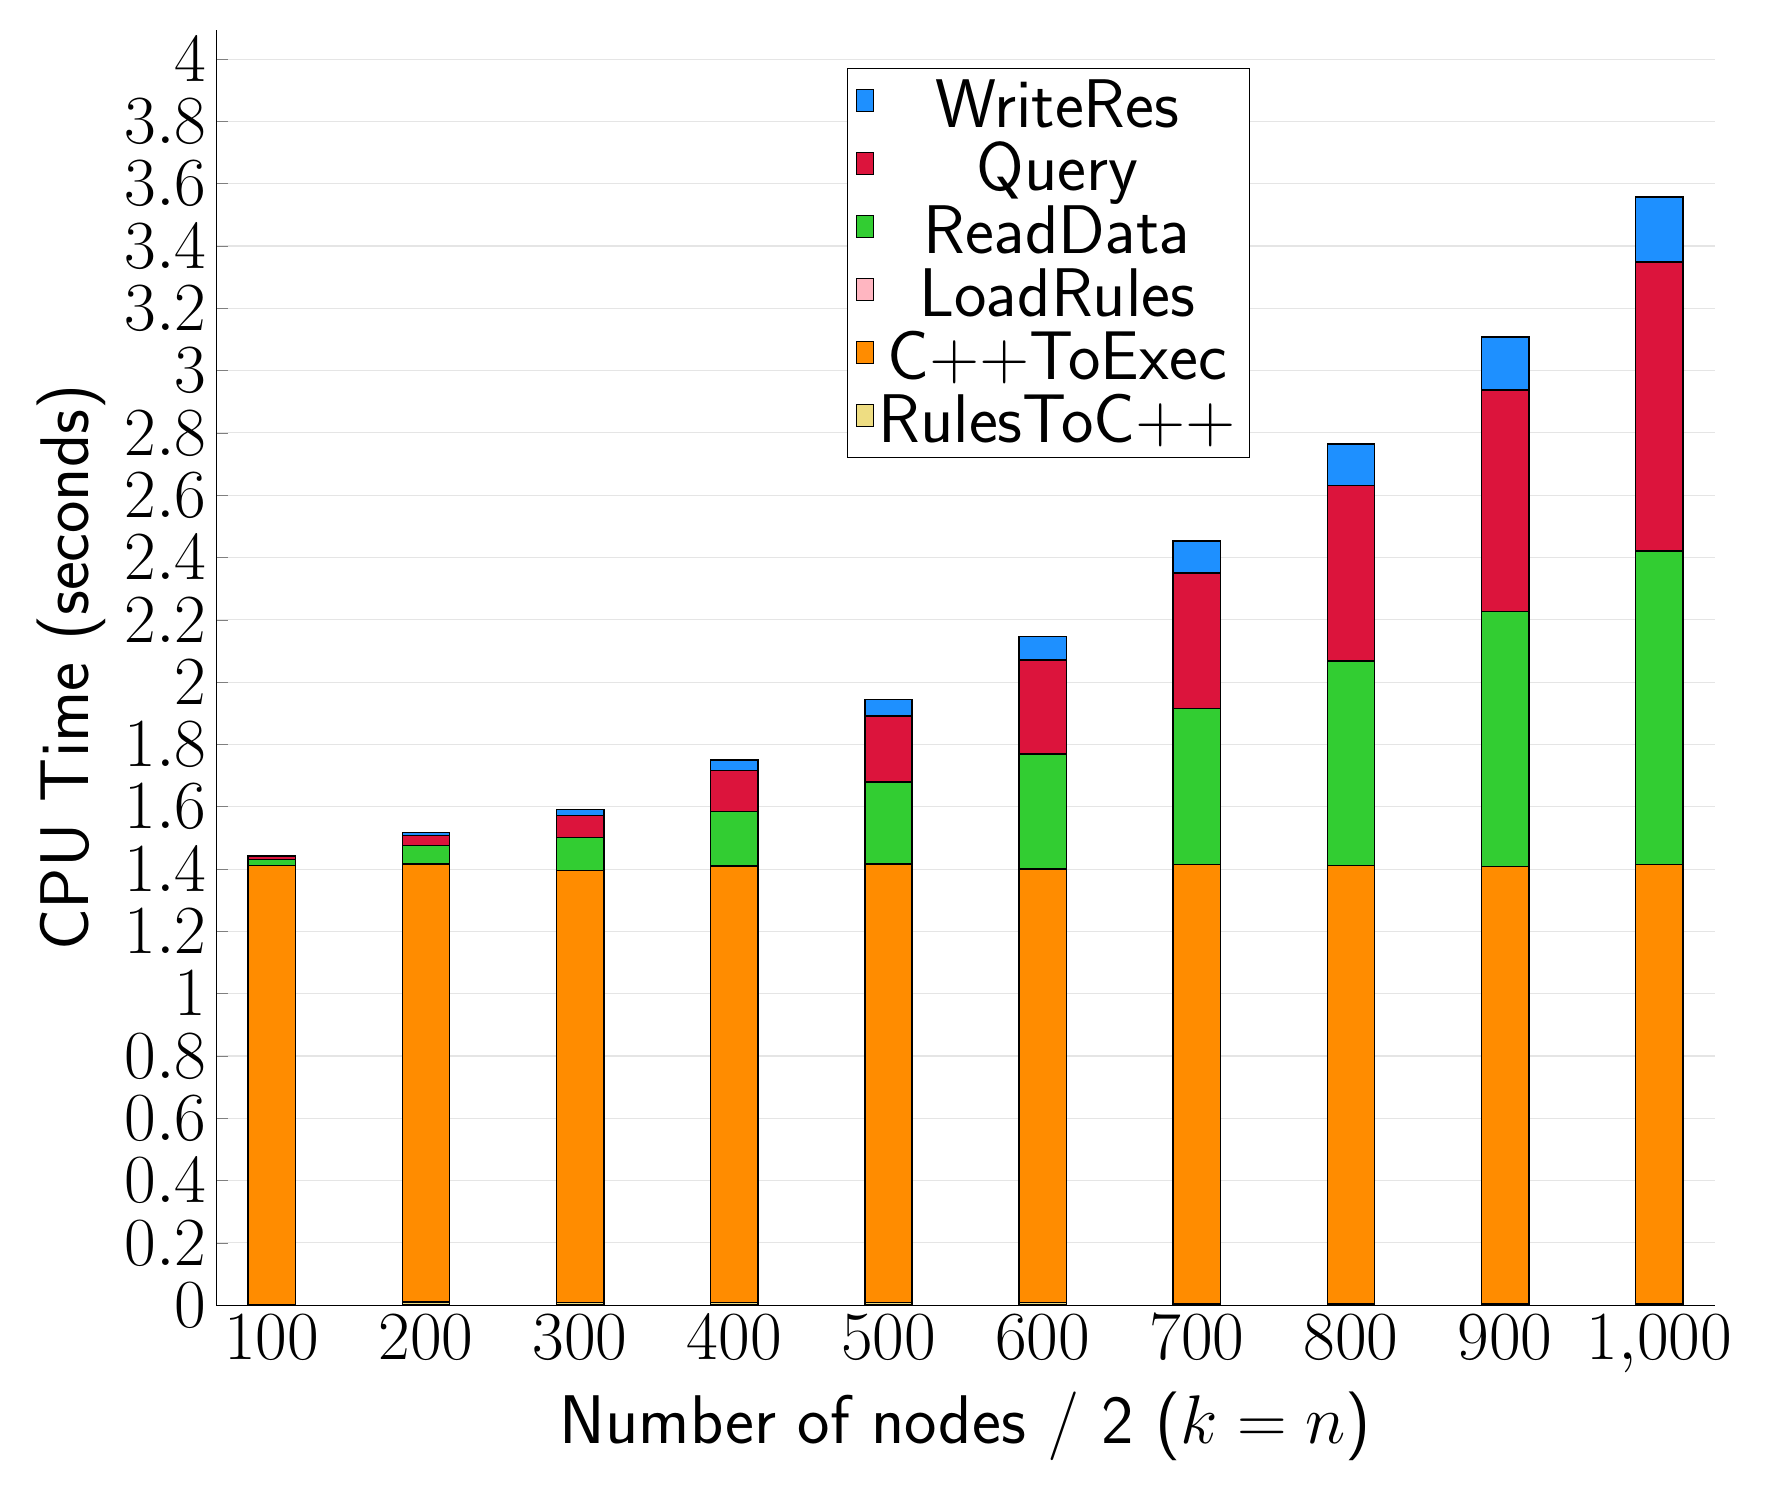
\begin{tikzpicture}
\begin{axis}[
   ybar stacked,
   width=1.7\textwidth,
   bar width=0.6cm,
   ymajorgrids, tick align=inside,
   major grid style={draw=gray!20},
   xtick=data,
   ymin=0, ymax=4.094,
   axis x line*=bottom,
   axis y line*=left,
   enlarge x limits=0.04,
   legend style={
       at={(0.69, 0.97)},
       anchor=north east,
       legend columns=1,
       font=\Huge,
   },
   ylabel={CPU Time (seconds)},
   xlabel={Number of nodes / 2 ($k=n$)},
   label style={font=\Huge},
   tick label style={font=\Huge},
]
\addlegendimage{fill=DodgerBlue, draw=black, line width=0.2pt}
\addlegendentry{WriteRes}
\addlegendimage{fill=Crimson, draw=black, line width=0.2pt}
\addlegendentry{Query}
\addlegendimage{fill=LimeGreen, draw=black, line width=0.2pt}
\addlegendentry{ReadData}
\addlegendimage{fill=LightPink, draw=black, line width=0.2pt}
\addlegendentry{LoadRules}
\addlegendimage{fill=DarkOrange, draw=black, line width=0.2pt}
\addlegendentry{C++ToExec}
\addlegendimage{fill=LightGoldenrod, draw=black, line width=0.2pt}
\addlegendentry{RulesToC++}
\addplot +[fill=LightGoldenrod, draw=black, line width=0.55pt] coordinates {
(100, 0.001999999999999999)
(200, 0.009999999999999995)
(300, 0.007999999999999997)
(400, 0.007999999999999997)
(500, 0.007999999999999988)
(600, 0.007999999999999997)
(700, 0.006)
(800, 0.005999999999999997)
(900, 0.003999999999999998)
(1000, 0.004000000000000001)
};
\addplot +[fill=DarkOrange, draw=black, line width=0.55pt] coordinates {
(100, 1.4100000000000001)
(200, 1.4060000000000001)
(300, 1.388)
(400, 1.4020000000000001)
(500, 1.4080000000000001)
(600, 1.392)
(700, 1.4080000000000001)
(800, 1.4060000000000001)
(900, 1.4040000000000004)
(1000, 1.4100000000000001)
};
\addplot +[fill=LightPink, draw=black, line width=0.55pt] coordinates {
(100, 0.00012880000000000001)
(200, 0.0001566)
(300, 0.00011200000000000001)
(400, 0.00013979999999999998)
(500, 0.0001394)
(600, 0.0001332)
(700, 0.0001482)
(800, 0.0001418)
(900, 0.0001014)
(1000, 9.4e-05)
};
\addplot +[fill=LimeGreen, draw=black, line width=0.55pt] coordinates {
(100, 0.018565599999999998)
(200, 0.059831199999999994)
(300, 0.10488220000000001)
(400, 0.17447759999999998)
(500, 0.2632832)
(600, 0.36911459999999996)
(700, 0.5014428)
(800, 0.6551052)
(900, 0.8189446)
(1000, 1.0060854)
};
\addplot +[fill=Crimson, draw=black, line width=0.55pt] coordinates {
(100, 0.0102292)
(200, 0.032230999999999996)
(300, 0.07124520000000001)
(400, 0.1322404)
(500, 0.2122284)
(600, 0.3023536)
(700, 0.4339588)
(800, 0.5632654)
(900, 0.7113028)
(1000, 0.9285596)
};
\addplot +[fill=DodgerBlue, draw=black, line width=0.55pt] coordinates {
(100, 0.0031597999999999995)
(200, 0.008653600000000001)
(300, 0.019287199999999997)
(400, 0.033961)
(500, 0.052140399999999996)
(600, 0.07539180000000001)
(700, 0.10312760000000001)
(800, 0.13431099999999999)
(900, 0.1700042)
(1000, 0.2081878)
};
\end{axis}
\end{tikzpicture}

\end{document}
